La vela major d'un veler té forma semiparabòlica i està delimitada per les gràfiques de $f(x)=-x^2+25$, $y=0$
i $x=0$, tal com s'indica a la figura següent:
\begin{center}
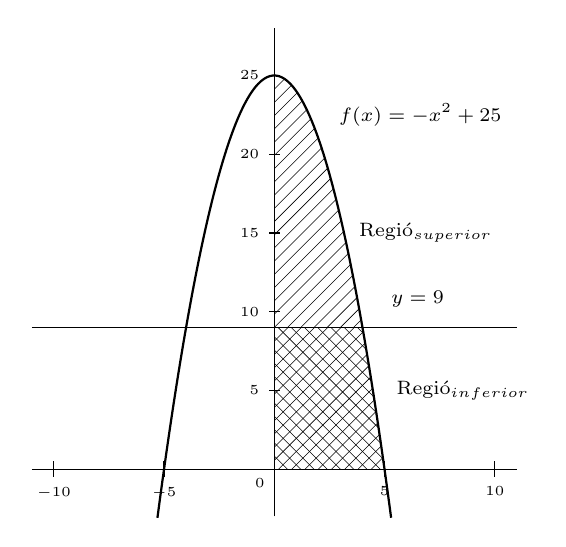
\begin{tikzpicture}[x=0.28cm,y=0.2cm]
  \begin{scope}
    \clip (0,9) -- (0,25) -- plot[domain=0:4,samples=40,smooth] (\x,{25-(\x)*(\x)}) -- (4,9) -- cycle;
    \foreach \t in {-12,-11.4,...,4.2} \draw[very thin] (\t,9) -- ++(12,16.8);
  \end{scope}
  \begin{scope}
    \clip (0,0) -- (0,9) -- (4,9) -- plot[domain=4:5,samples=20,smooth] (\x,{25-(\x)*(\x)}) -- (5,0) -- cycle;
    \foreach \t in {-7,-6.4,...,6} \draw[very thin] (\t,0) -- ++(7,9.8);
    \foreach \t in {0,0.6,...,12} \draw[very thin] (\t,0) -- ++(-7,9.8);
  \end{scope}
  \draw (-11,0) -- (11,0);
  \draw (0,-3) -- (0,28);
  \foreach \i in {-10,-5,5,10} \draw (\i,0.5) -- (\i,-0.5) node[below,font=\tiny] {$\i$};
  \node[below left,font=\tiny] at (0,0) {$0$};
  \foreach \j in {5,10,15,20,25} \draw (0.25,\j) -- (-0.25,\j) node[left,font=\tiny] {$\j$};
  \draw (-11,9) -- (11,9);
  \draw[\colorgrafica,thick,domain=-5.3:5.3,samples=80,smooth] plot (\x,{25-(\x)*(\x)});
  \node[right,font=\scriptsize] at (2.5,22.5) {$f(x)=-x^2+25$};
  \node[right,font=\scriptsize] at (3.4,15) {Regió$_{\text{superior}}$};
  \node[font=\scriptsize] at (6.5,10.8) {$y=9$};
  \node[right,font=\scriptsize] at (5.1,5) {Regió$_{\text{inferior}}$};
\end{tikzpicture}
\end{center}
La vela té dues parts separades per la recta $y=9$. Per a construir-la, s'empra un teixit de niló a la part
superior, que costa $50\ \text{€}/\text{u}^2$, i un teixit de polièster a la part inferior, que costa
$70\ \text{€}/\text{u}^2$.

\begin{apartats}

\apartat{2,5}
Calculeu el cost total del material que es necessita per a construir aquesta vela.

\begin{solucio}
La vela ocupa la regió compresa entre les corbes $y=0$, $x=0$ i $y=-x^2+25$. Per calcular el cost total,
caldrà calcular separadament l'àrea de la regió superior i l'àrea de la regió inferior, i multiplicar-les
cadascuna pel preu del material respectiu (niló o polièster).\\
Trobem primer els punts de tall entre les funcions involucrades. El punt de tall de $y=-x^2+25$ amb la part
positiva de l'eix d'abscisses és $y=0\rightarrow-x^2+25=0\rightarrow x=5$. L'abscissa positiva del punt de
tall entre les corbes $y=-x^2+25$ i $y=9$ és $-x^2+25=9\rightarrow-x^2=-16\rightarrow x=4$.\\
L'àrea total sota la corba $y=-x^2+25$ entre els extrems $x=0$ i $x=5$ és
\[
A_{\text{total}}=\int_0^5\left(-x^2+25\right)dx=\left[-\frac{x^3}{3}+25x\right]_0^5=-\frac{125}{3}+125-0
=\frac{250}{3}\ \text{u}^2 .
\]
L'àrea de la regió inferior és
\begin{align*}
A_{\text{inf}}&=\int_0^4 9\,dx+\int_4^5\left(-x^2+25\right)dx=9\cdot4+\left[-\frac{x^3}{3}+25x\right]_4^5\\
&=36+\left(-\frac{125}{3}+125\right)-\left(-\frac{64}{3}+100\right)=36+\frac{14}{3}=\frac{122}{3}\ \text{u}^2 .
\end{align*}
Finalment, l'àrea de la regió superior és la diferència:
$A_{\text{sup}}=A_{\text{total}}-A_{\text{inf}}=\frac{250}{3}-\frac{122}{3}=\frac{128}{3}\ \text{u}^2$.\\
Així doncs, el cost total de la vela serà
\begin{align*}
&\frac{128}{3}\ \text{u}^2\cdot50\ \text{€}/\text{u}^2+\frac{122}{3}\ \text{u}^2\cdot70\ \text{€}/\text{u}^2\\
&\qquad=\frac{6\,400+8\,540}{3}\ \text{€}=4\,980\ \text{€}.
\end{align*}

\textit{Pauta oficial:} 0,25 pels punts de tall; 0,5 pel plantejament de l'àrea de la regió inferior, i 0,5
pel càlcul; 0,5 pel plantejament de l'àrea de la regió superior, i 0,5 pel càlcul, i, finalment, 0,25 pel
càlcul del cost final. Hi ha altres maneres de plantejar el càlcul de les dues àrees: compteu-les bé si ho
fan correctament i de manera justificada.
\end{solucio}

\end{apartats}
